\chapter{Ensayos y resultados}

\label{Chapter4}

En este capítulo se describen los ensayos llevados a cabo para verificar que todos los requisitos del proyecto fueron cumplidos.

\section{Ensayos de verificación}

Se ensambló un banco de ensayos para poder evaluar el rendimiento del sistema y resolver los fallos que ocurrieron durante el desarrollo. De esta forma se evitó la dependencia de disponer un motor de combustión interna para los ensayos. Las figuras \ref{fig:banco-pruebas-1} y \ref{fig:banco-pruebas-2} muestran dicho banco de pruebas durante uno de ellos.

\begin{figure}[htpb]
\centering
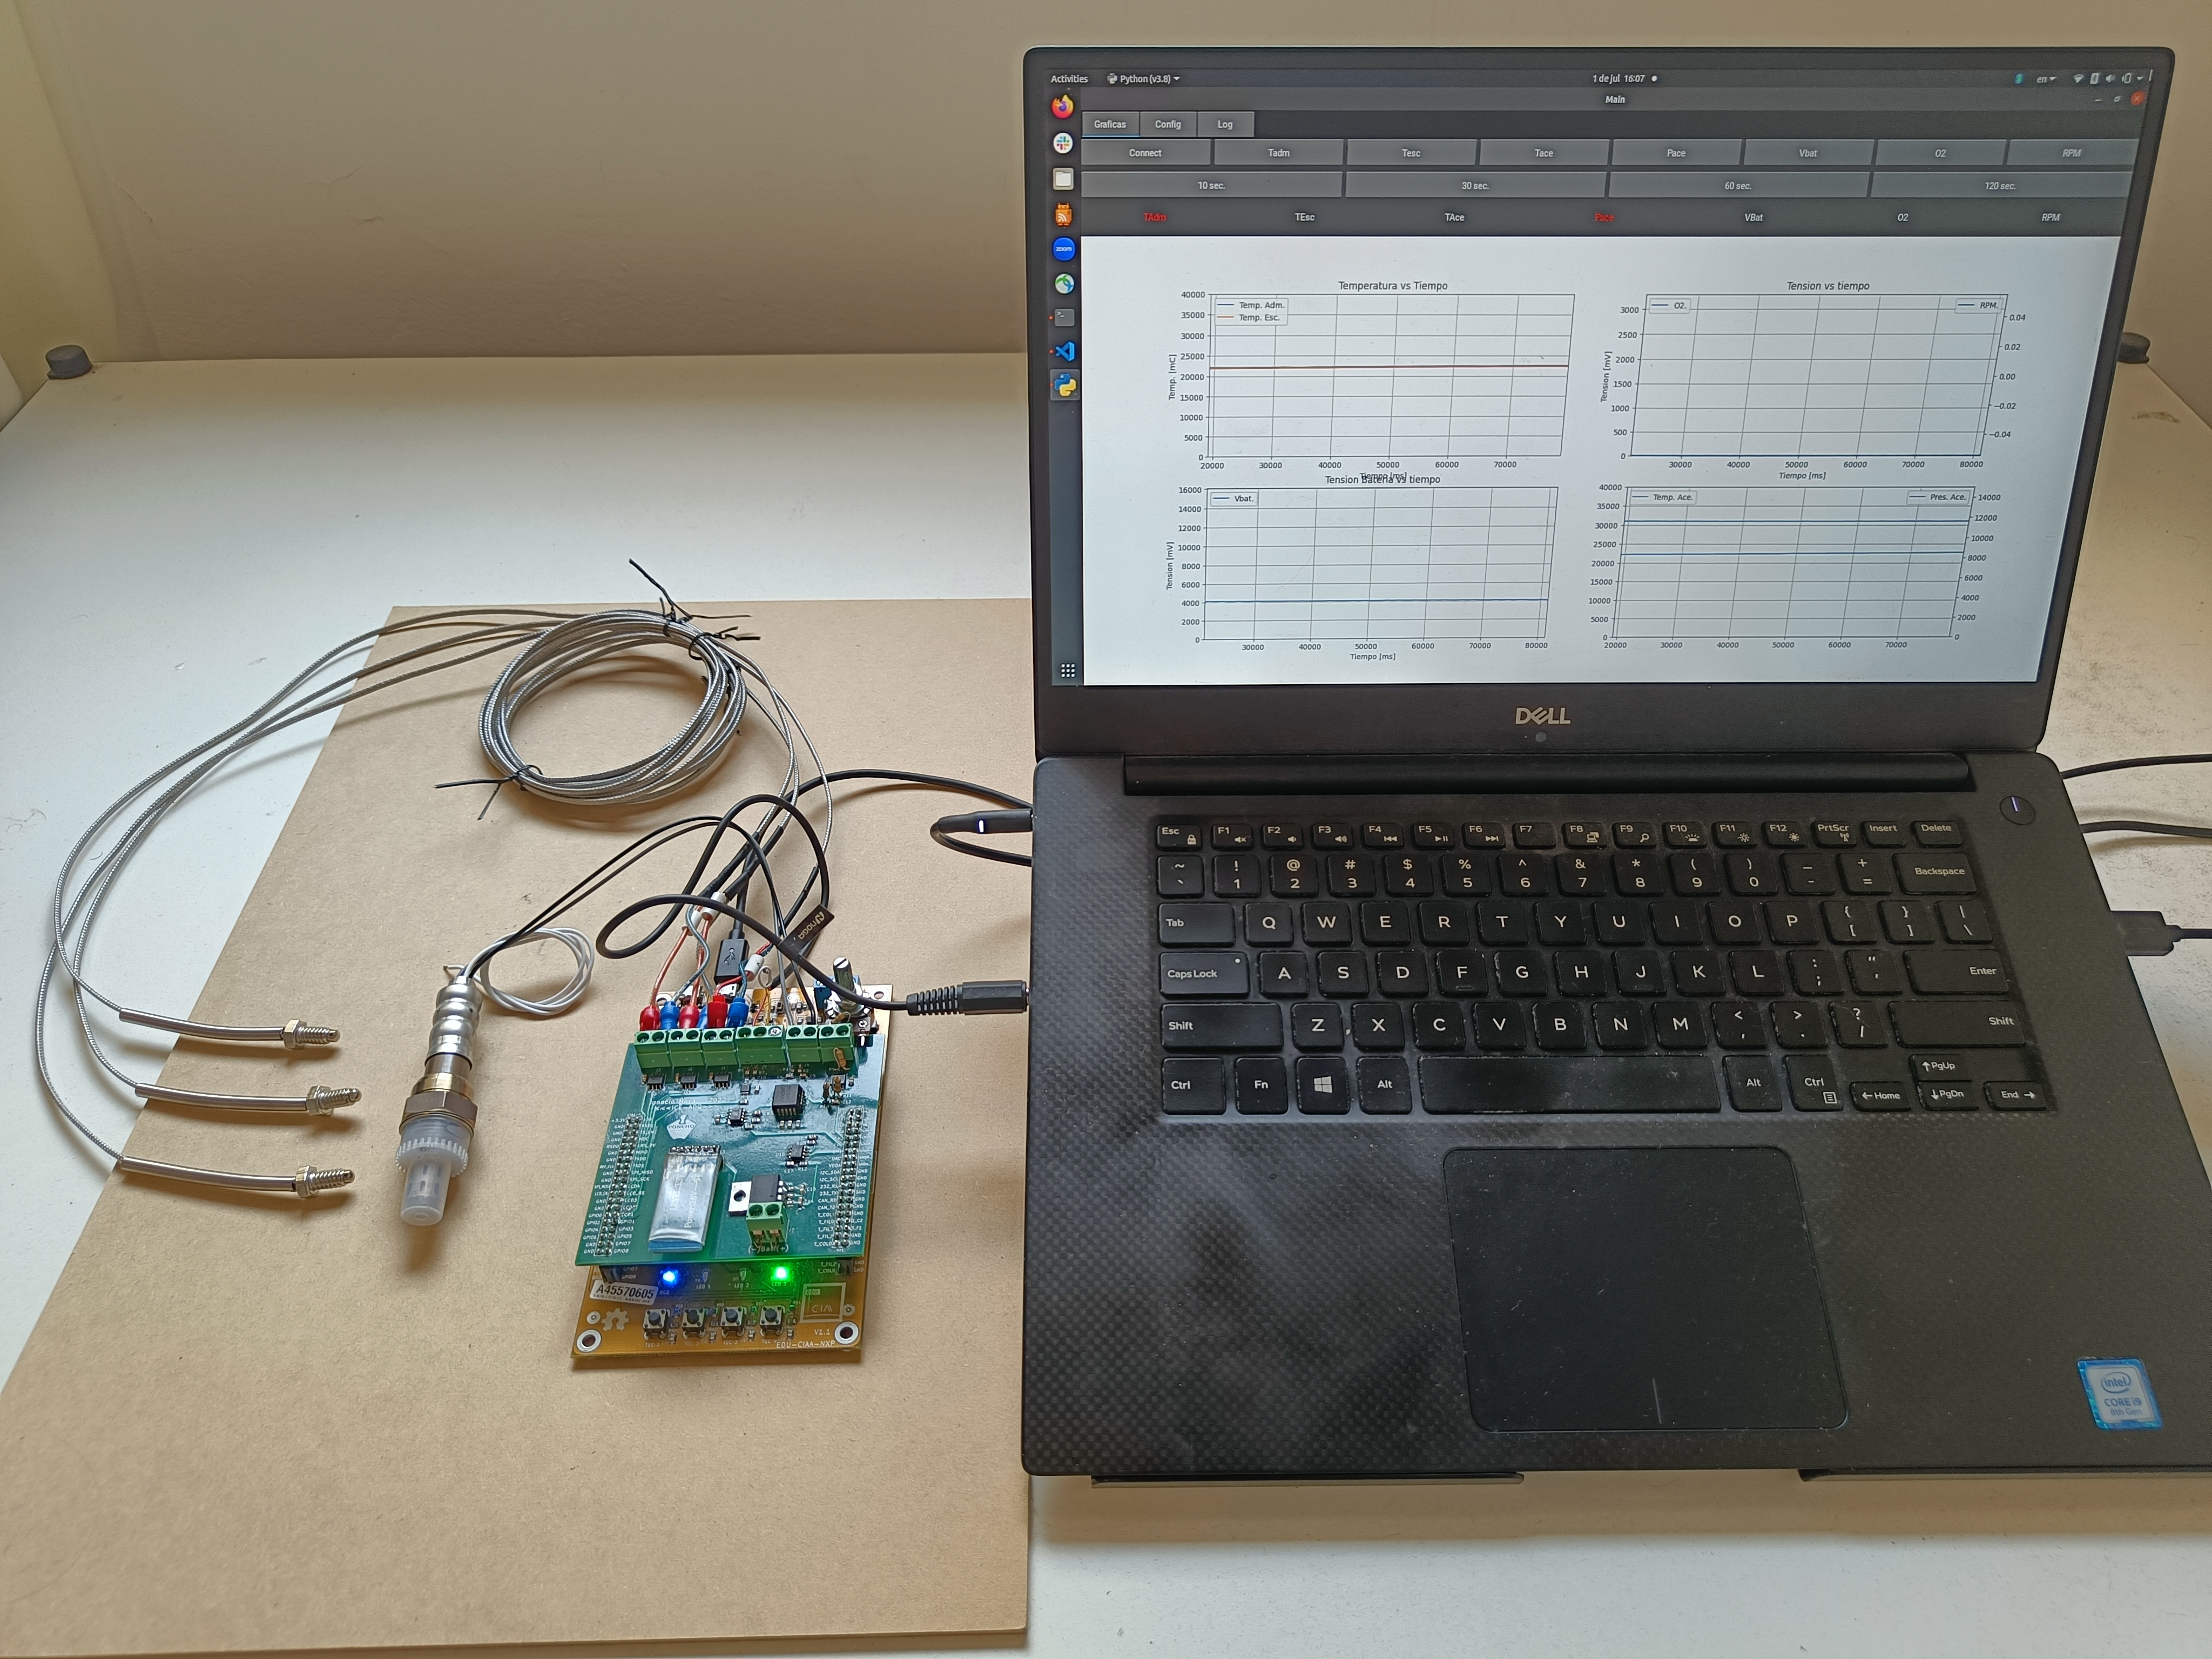
\includegraphics[width=.85\textwidth]{./Figures/banco-pruebas-1.jpg}
\caption{Fotografía del banco de pruebas en uso durante uno de los ensayos.}
\label{fig:banco-pruebas-1}
\end{figure}

\begin{figure}[htpb]
\centering
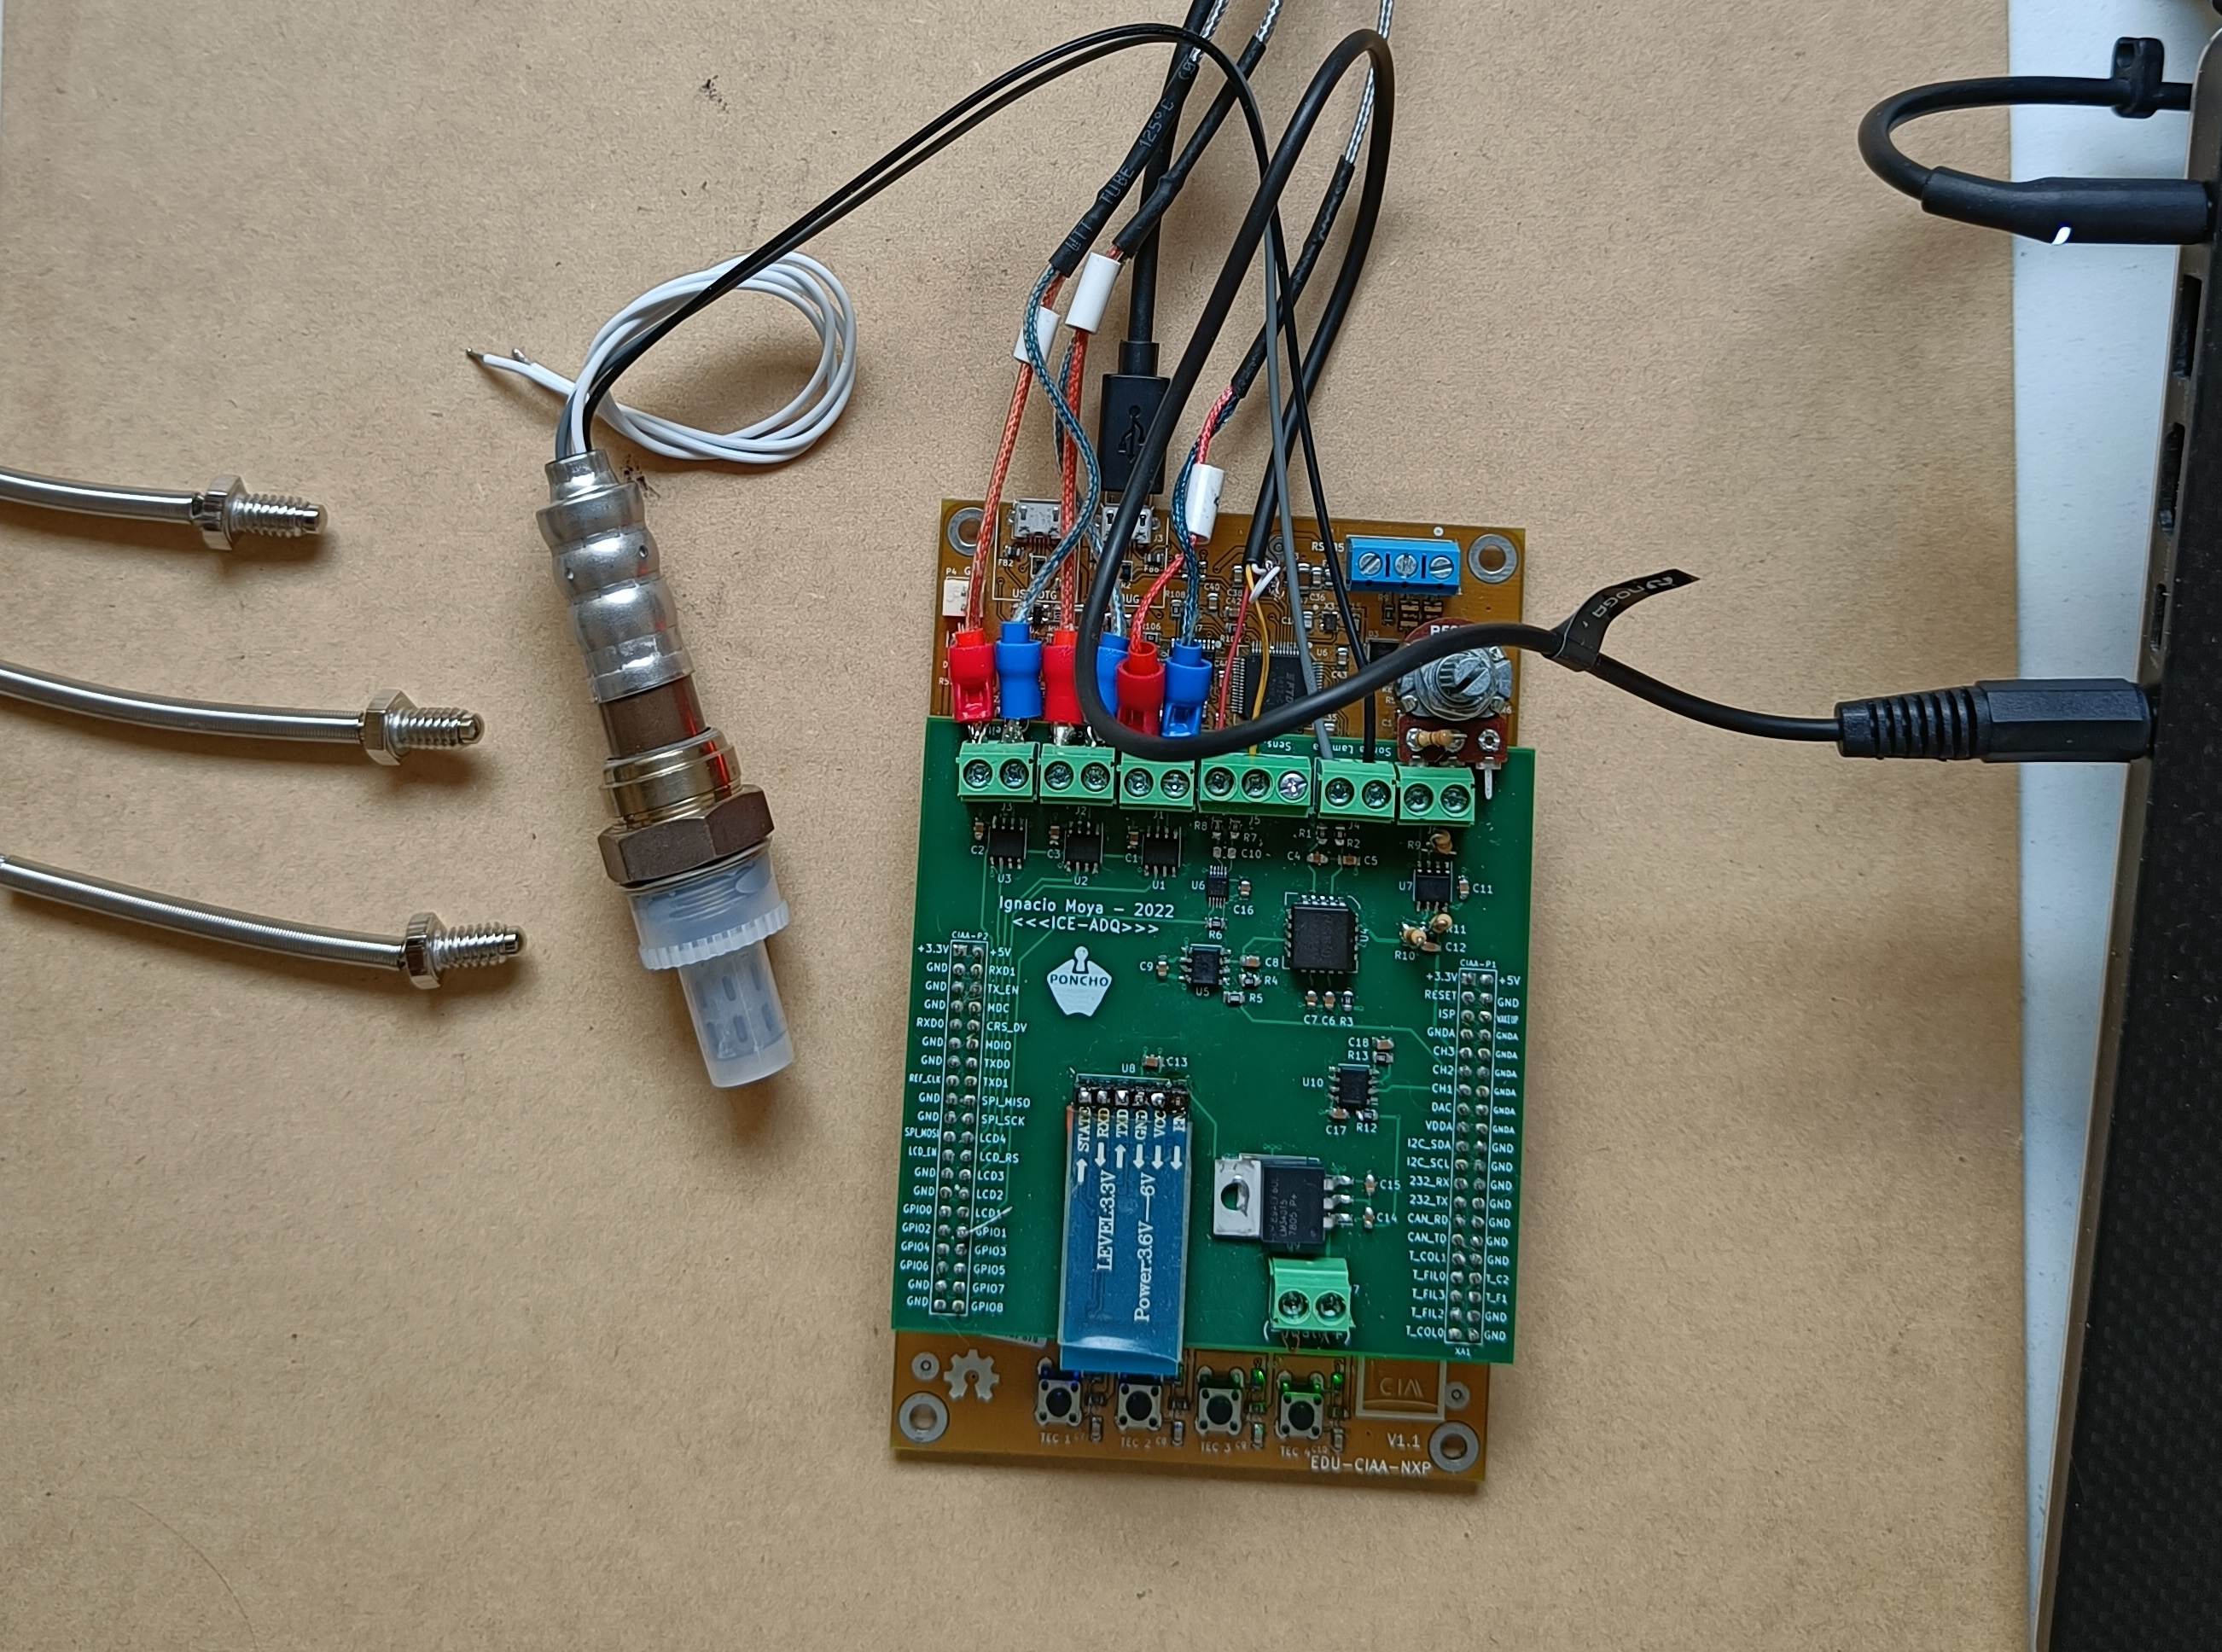
\includegraphics[width=.85\textwidth]{./Figures/banco-pruebas-2.jpg}
\caption{Fotografía en detalle del circuito impreso montado sobre la EDU-CIAA y con sensores conectados.}
\label{fig:banco-pruebas-2}
\end{figure}
\break
\subsection{Ensayos de medición de temperatura}

Se contrastaron las mediciones realizadas por el sistema contra las mediciones realizadas por un multímetro que tiene medición de termocupla tipo K. Para la contrastación se sumergieron a todas las termocuplas en un recipiente con agua, el ensayo se repitió tres veces y en estas reiteraciones la temperatura del agua fue de 0 \degree C, 100 \degree C y 20 \degree C considerada temperatura ambiente.

\begin{table}[htpb]
	\centering
	\caption{Resultados de ensayo a 0 \degree C.}
	\centering
	\begin{tabular}{l c}    
		\toprule
		\textbf{Sensor }     & \textbf{Lectura [\degree C]} \\
		\midrule
		Termocupla admisión		&   0,25 \\
		Termocupla escape		&   0,50 \\
		Termocupla aceite		& - 0,25 \\
		Termocupla contraste	&   0,03 \\
		\bottomrule
	\end{tabular}
	\label{tab:ensayo-0-degree}
\end{table}

\begin{table}[htpb]
	\centering
	\caption{Resultados de ensayo a 20 \degree C.}
	\centering
	\begin{tabular}{l c}    
		\toprule
		\textbf{Sensor }     & \textbf{Lectura [\degree C]} \\
		\midrule
		Termocupla admisión		&   20,25 \\
		Termocupla escape		&   20,75 \\
		Termocupla aceite		&   20,50 \\
		Termocupla contraste	&   19,95 \\
		\bottomrule
	\end{tabular}
	\label{tab:ensayo-20-degree}
\end{table}

\begin{table}[htpb]
	\centering
	\caption{Resultados de ensayo a 100 \degree C.}
	\centering
	\begin{tabular}{l c}    
		\toprule
		\textbf{Sensor }     & \textbf{Lectura [\degree C]} \\
		\midrule
		Termocupla admisión		&   100,50 \\
		Termocupla escape		&   100,75 \\
		Termocupla aceite		&   100,75 \\
		Termocupla contraste	&   100,50 \\
		\bottomrule
	\end{tabular}
	\label{tab:ensayo-100-degree}
\end{table}

En las tablas \ref{tab:ensayo-0-degree} , \ref{tab:ensayo-20-degree}, y \ref{tab:ensayo-100-degree} se listan los resultados de los tres ensayos de temperatura. A partir de dichos resultados se puede concluir que se cumplieron los requisitos REQ-ADQ-001 y REQ-ADQ-002.

\subsection{Ensayos de medición de presión de aceite}

Para verificar que la medición de presión de aceite cumpliera con el requisito REQ-ADQ-005 se realizaron dos ensayos distintos.

En el primero se simuló al sensor de presión con un potenciómetro de valor similar. Luego se midió la tensión en los contactos de la bornera en donde se conecta el sensor con el circuito impreso. Y, finalmente, se contrastó el valor de tensión medido, con la lectura realizada por el ADC, para ver en cuanto diferían entre si.

Para el segundo ensayo, se conectó al sensor de presión a una bomba de presión de aire manual con manómetro integrado, para simular así la presión del fluído y contrastar el valor medido con la lectura del manómetro.

\subsection{Ensayos de medición de velocidad de giro}

El ensayo de verificación de medición de velocidad de giro, se realizó simulando al sensor de reluctancia variable, con la placa de sonido de una computadora. A través de un software generador de señales, se inyectó en la entrada del circuito una señal triangular de frecuencia variable y de amplitud de 1 Vp2p. Este ensayo se basó de la hoja de datos del kit de evaluación del MAX9924 \cite{max9924evk}. Al igual que indica la hoja de datos del kit de evaluación, se hicieron ensayos con cuatro valores de frecuencia diferentes, 5 Hz, 55Hz, 2,5 kHz y 24 kHz.

Como se puede observar de los resultados del ensayo listados en la tabla \ref{tab:ensayo-rpm}, el prototipo cumple con el requisito REQ-ADQ-003.

\begin{table}[htpb]
	\centering
	\caption{Resultados de ensayo de medición de velocidad de giro.}
	\centering
	\begin{tabular}{c c}    
		\toprule
		\textbf{Frecuencia señal }     & \textbf{Lectura} \\
		\midrule
		5 Hz		&   5,1 Hz \\
		55 Hz		&   54,9 Hz \\
		2500 Hz		&   2499,9 Hz \\
		24000 Hz	&   2399,9 Hz \\
		\bottomrule
	\end{tabular}
	\label{tab:ensayo-rpm}
\end{table}

\subsection{Ensayos de medición de la sonda lambda}

Ante la falta de un dispositivo capaz de leer una sonda lamba para luego contrastar su lectura. Se optó por realizar una lectura indirecta del sensor, midiendo la tensión en bornes del mismo. Luego, se contrastó la lectura realizada por el prototipo, con el resultado de calcular el factor lambda correspondiente a la tensión en bornes medida.

\subsection{Ensayo de pérdida de paquetes}

Para este ensayo se modificó el software de ambas partes del sistema para agregar un campo extra a cada paquete transmitido para enumerar a cada uno de ellos con un número que comienza en 0 y se incrementa por 1 cada vez que se transmite un paquete. De esta forma es posible saber si existió pérdida de paquetes durante la transmisión verificando que la secuencia de los números no se vio interrumpida al finalizar el ensayo. Luego se colocaron ambas partes separadas por una distancia de tres metros y se inició la trasmisión de información hasta llegar a la cantidad de 10.000 paquetes transmitidos. 

Resultado: No se encontró pérdida de datos después de 10.000 transmisiones consecutivas, se verificó que el requisito REQ-COMM-001 fue cumplido.

\subsection{Ensayo de tiempo de transmisión}


\section{Casos de uso}

En esta sección se describen los casos de uso utilizados para ensayar si la interfaz gráfica cumple con los requisitos

\begin{table}
	\centering
	\caption{Caso de uso de conectarse a la parte adquisidora.}
	\centering
	\begin{tabular}{c c}    
		\toprule
		\textbf{Título }     & \textbf{Descripción} \\
		\midrule
		Identificador		&  CU1. \\
		Nombre				&   Conectarse a parte adquisidora. \\
		Actor principal		&   Usuario \\
		Disparadores		&   El usuario presiona el botón "Conectar" \\
		Flujo básico		&   \\
		Pre-condiciones		&   La parte adquisidora tiene que estar funcionamiento y su LED azul parpadeando. \\
		Post-condiciones	&   \\
		\bottomrule
	\end{tabular}
\label{tab:caso-conectar}
\end{table}

\begin{table}
	\centering
	\caption{Caso de uso de ocultar una variable de su gráfica.}
	\centering
	\begin{tabular}{c c}    
		\toprule
		\textbf{Título }     & \textbf{Descripción} \\
		\midrule
		Identificador		&  CU2. \\
		Nombre				&   Ocultar variable en la gráfica. \\
		Actor principal		&   Usuario \\
		Disparadores		&   El usuario presiona el botón que tiene el mismo nombre de la variable que quiere ocultar. \\
\\
		Pre-condiciones		&   La variable se encuentra visible. \\
		Post-condiciones	&   La variable deja de estar visible.\\
		\bottomrule
	\end{tabular}
\label{tab:caso-ocultar}
\end{table}

\begin{table}
	\centering
	\caption{Caso de uso de mostrar una variable oculta.}
	\centering
	\begin{tabular}{c c}    
		\toprule
		\textbf{Título }     & \textbf{Descripción} \\
		\midrule
		Identificador		&	CU3. \\
		Nombre				& 	Mostrar variable oculta. \\
		Actor principal		&   Usuario \\
		Disparadores		&   El usuario presiona el botón que tiene el mismo nombre de la variable que quiere mostrar. \\
\\
		Pre-condiciones		&   La variable se encuentra oculta. \\
		Post-condiciones	&   La variable es visualizada en su gráfica correspondiente.\\
		\bottomrule
	\end{tabular}
\label{tab:caso-mostrar}
\end{table}


